\begin{comment}


\begin{refsection}

    \chapter{Engineering supramolecular networks using Ch-bonding}
    
    \section{Introduction}
    
    \begin{figure}
        \replacecmpd{ebs.3py}
        \replacecmpd{ebs.3pyme}
        \replacecmpd{ebs.3pyhcl}
        \replacecmpd{selenylchloride-3py}
        \centering
        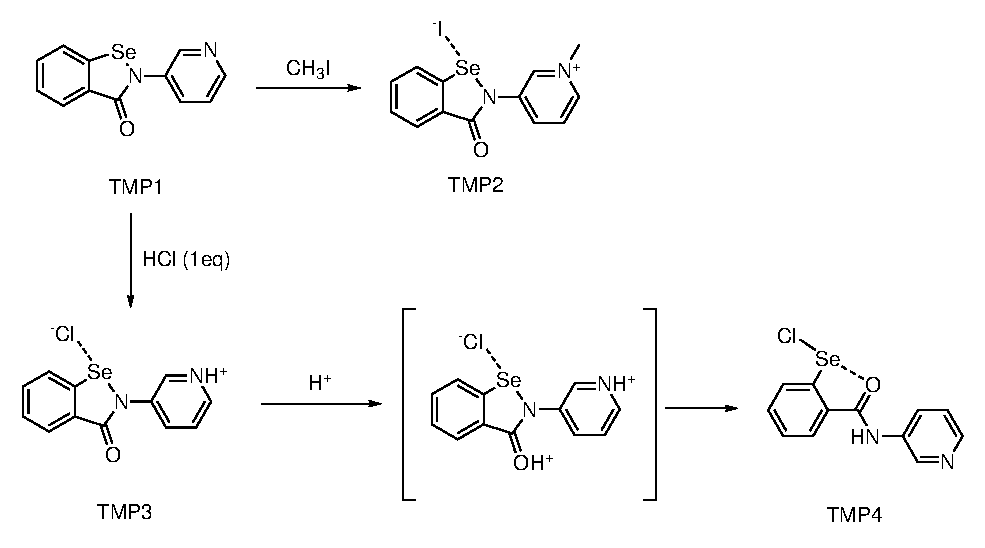
\includegraphics[scale=0.74]{Figures/ebs-3py-scheme.eps}
        \caption{Reactions of 3-pyridyl ebselen \refcmpd{ebs.3py}.}
        \label{sch:selenylchloride-mechanism}
    \end{figure}
    
    We prepared a 3-pyridyl ebselen derivative \cmpd{ebs.3py} in the hope that it would form a one-dimensional network consisting of linear Ch-bonded chains, and we were pleased to find that this was indeed the case.\autocite{???}
    
    In the crystal packing of \cmpd{ebs.3py}, each molecule is Ch-bonded through the pyridyl nitrogen to an adjacent molecule generated by the \textit{n}-glide, with a \ce{Se\dots N} distance of 2.386(1)~\AA.
    There is an additional Ch-bond to the carbonyl oxygen of the molecule generated by the \textit{n}-glide plus a translation along the \textit{a} axis (\cref{fig:3py-ebs-chbonds}).
    The \ce{Se\dots O} distance is 3.336(1)~\AA.
    The bond angles in both cases are consistent with a Ch-bonding interaction, with the nitrogen and oxygen atoms sitting almost perfectly opposite to the electron withdrawing group (174.43(5)\degree~and 165.89(4)\degree~respectively.)
    The $sp^2$ lone pairs of the nitrogen and oxygen atoms are also well aligned, at angles of 120.60(9)\degree~and 113.93(9)\degree~respectively.
    
    \begin{figure}
        \centering
        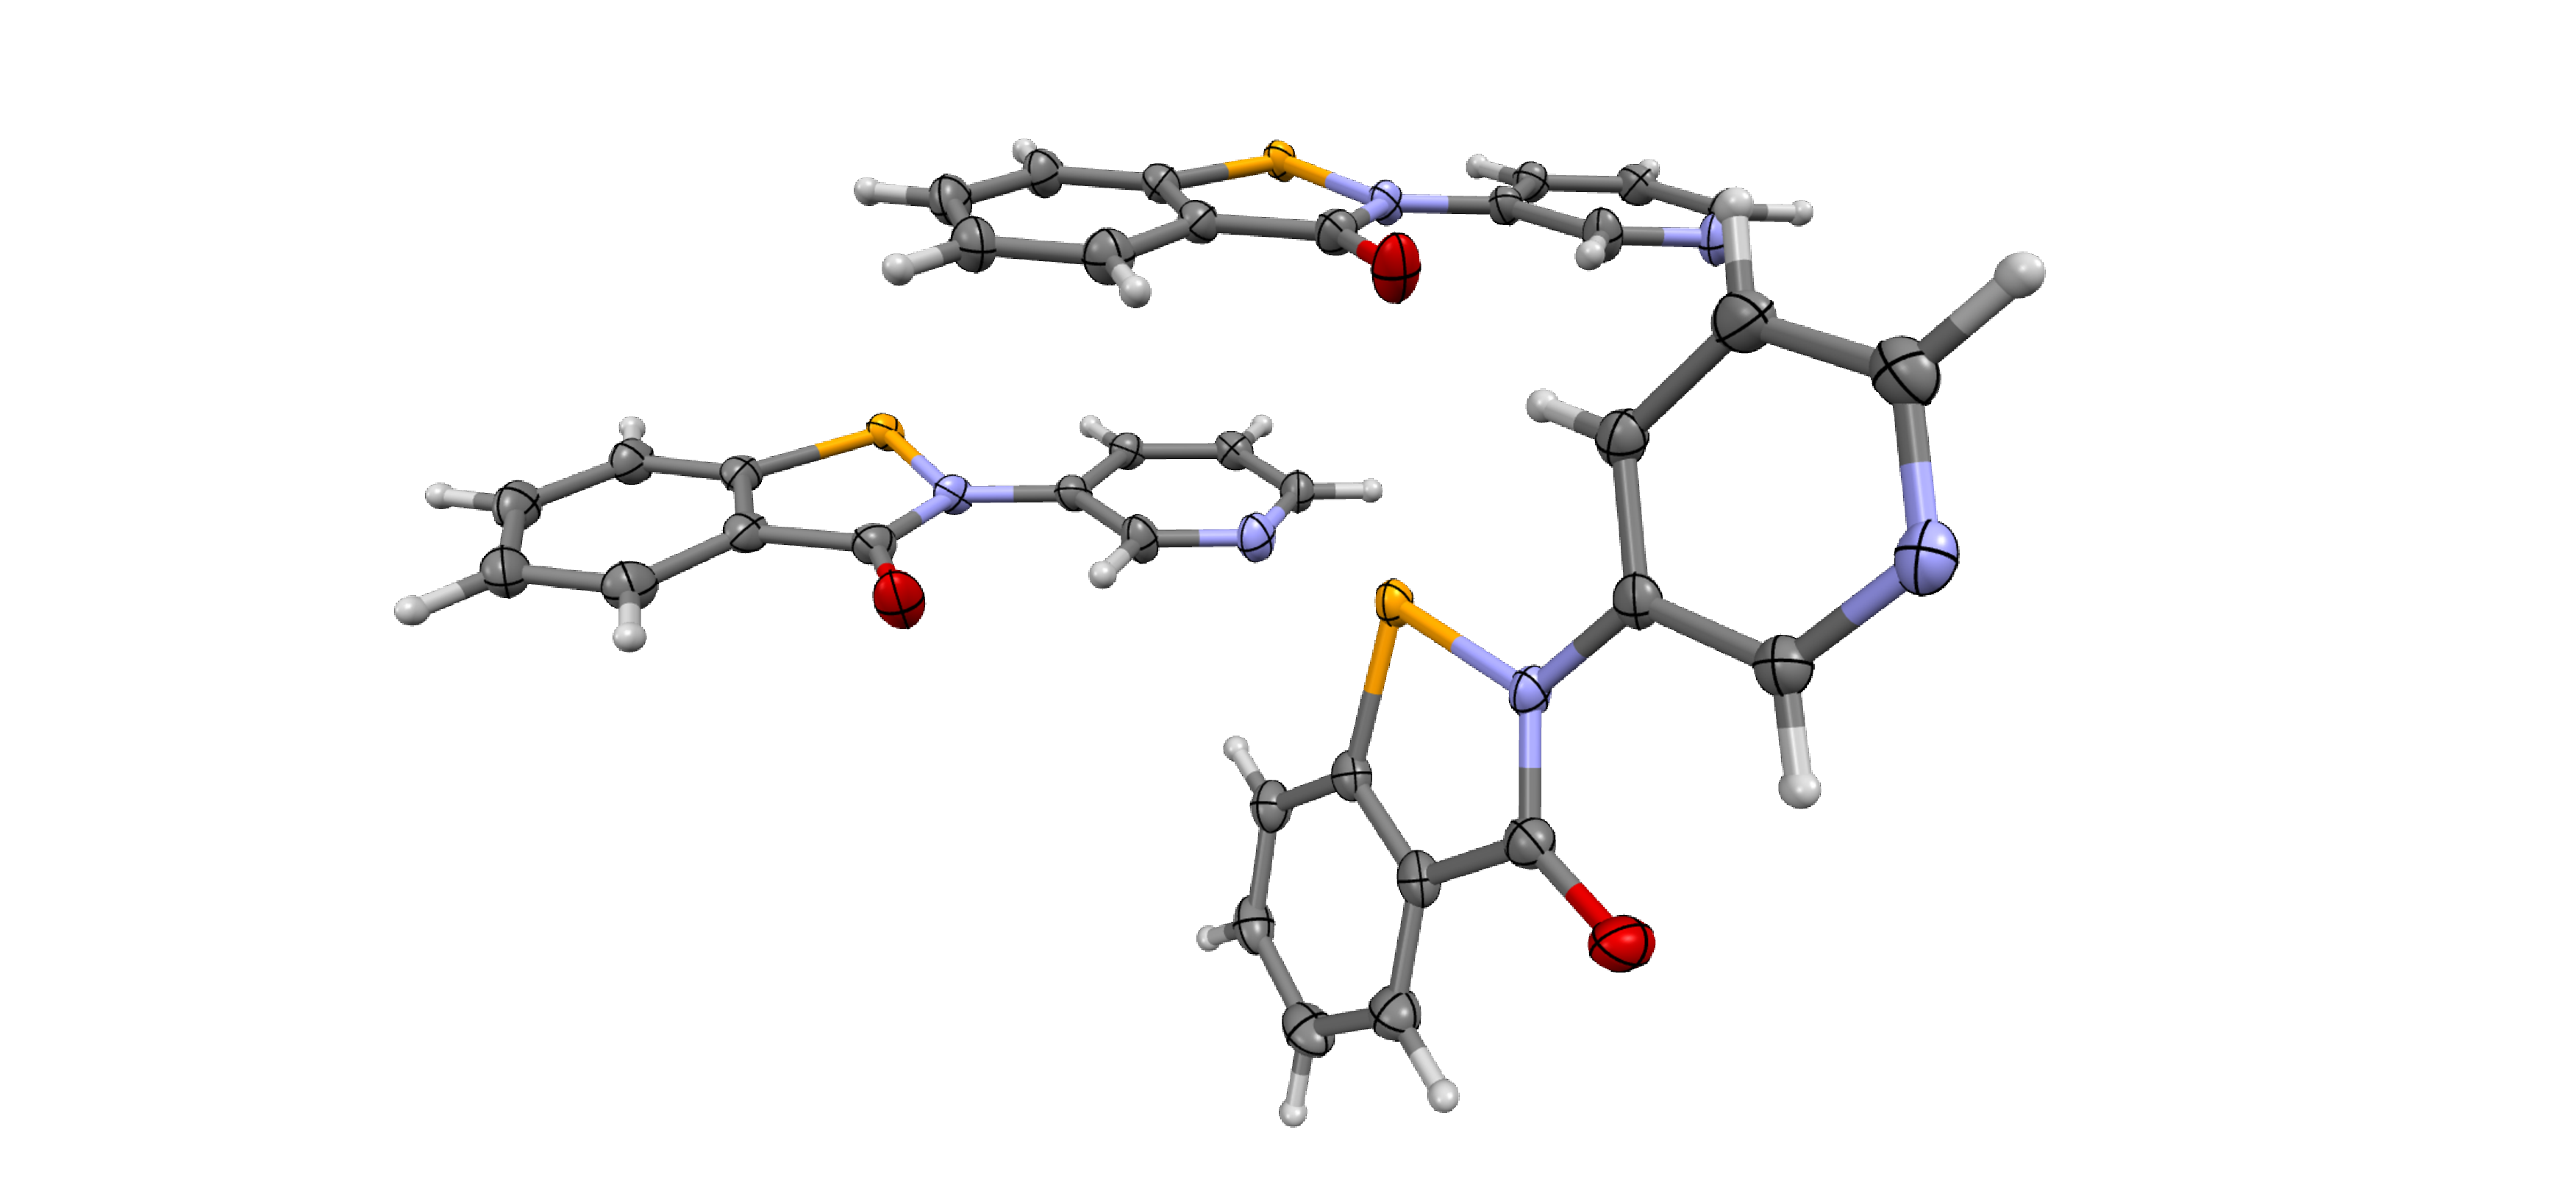
\includegraphics[width=\linewidth]{Figures/3py-ebs-chbonds.pdf}
        \caption[Ch-bonds formed by 3-pyridyl ebselen \refcmpd{ebs.3py} in the crystal packing.]{Ch-bonds formed by 3-pyridyl ebselen \refcmpd{ebs.3py} in the crystal packing. The stronger of the two is defined by the \ce{N-Se\cdots N_{pyr}} angle, and the weaker is defined by the \ce{C-Se\cdots O} angle.}
        \label{fig:3py-ebs-chbonds}
    \end{figure}
    
    \begin{figure}
        \centering
        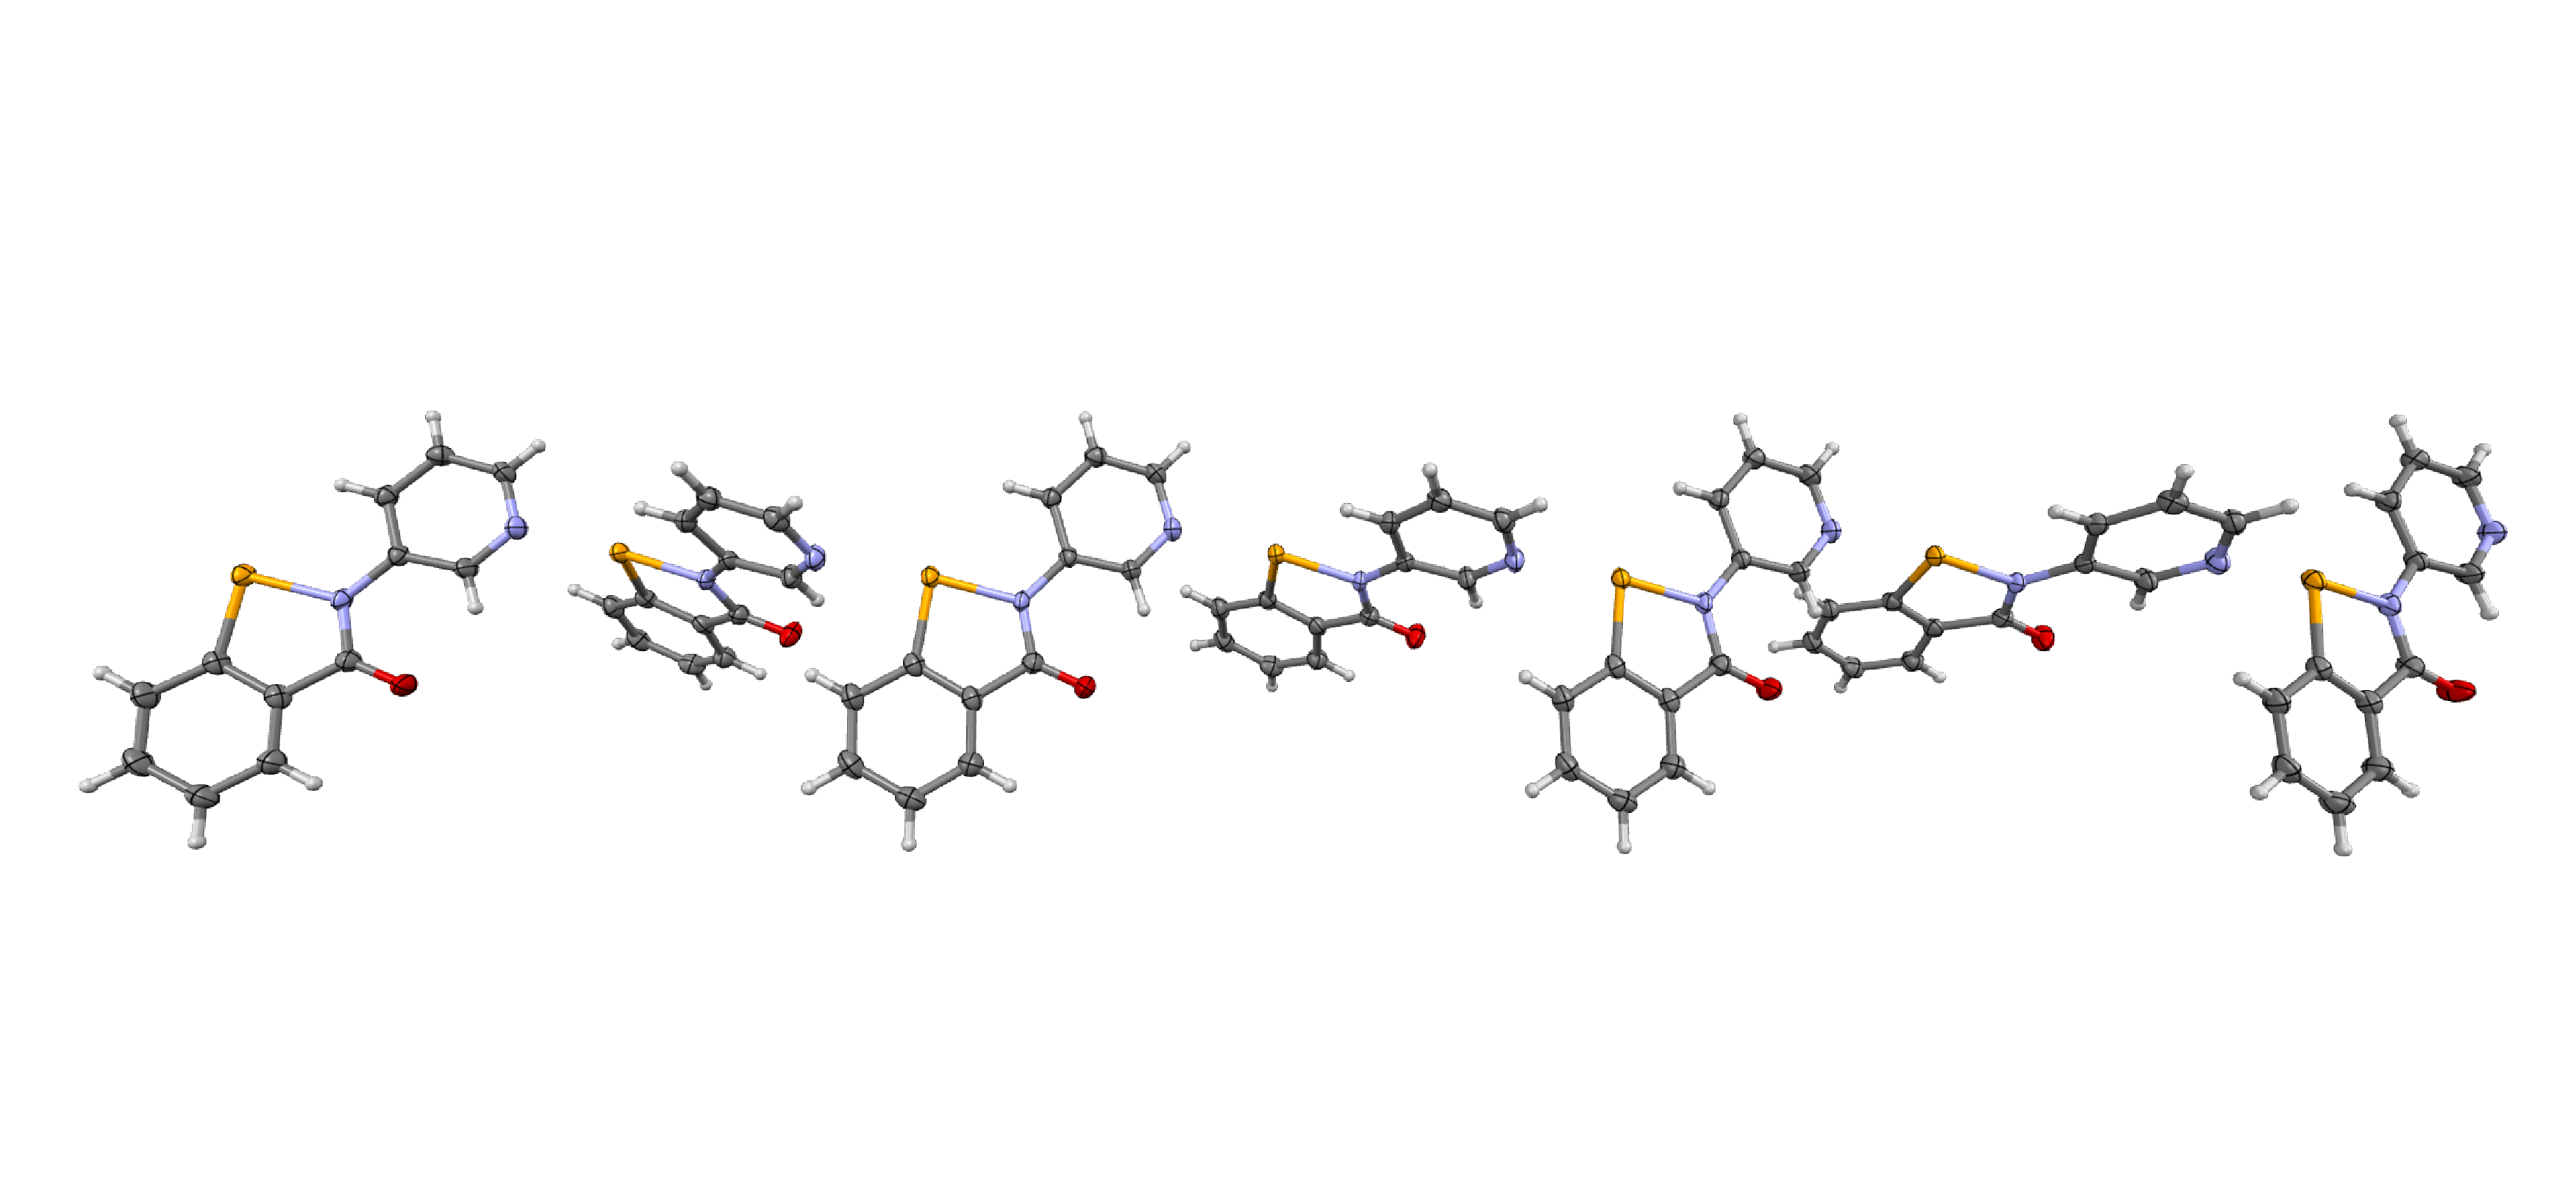
\includegraphics[width=\linewidth]{Figures/3py-ebs-chain.pdf}
        \caption[One-dimensional network formed by strong \ce{N-Se\dots N} Ch-bonds.]{One-dimensional network formed by strong \ce{N-Se\dots N} Ch-bonds. This is extended into 3 dimensions by the weaker \ce{C-Se\dots O} Ch-bonds, and $\pi$-stacking.}
        \label{fig:3py-ebs-chain}
    \end{figure}
    
    We have previously reported an instance of H-bond assisted Ch-bonding, in which a H-bond to the carbonyl of ebselen strengthens the resulting Ch-bond.
    We were interested to see if the introduction of a full positive charge in the molecule would have a similar effect, by analogy with charge-assisted H- and X-bonding.
    We therefore alkylated \cmpd{ebs.3py} using methyl iodide to form \cmpd{ebs.3pyme}, and were pleased to see yellow needles form in the reaction mixture almost immediately upon cooling.
    The structure of these crystals is shown in \cref{fig:3py-ebs-mei}.
    The pyridyl nitrogen is alkylated as expected, and the charge is balanced by the iodide Ch-bonded to the selenium, at a distance of 2.9904(4)~\AA~and an angle of 178.7(1)\degree~to the antipodal nitrogen.
    
    \begin{figure}
        \centering
        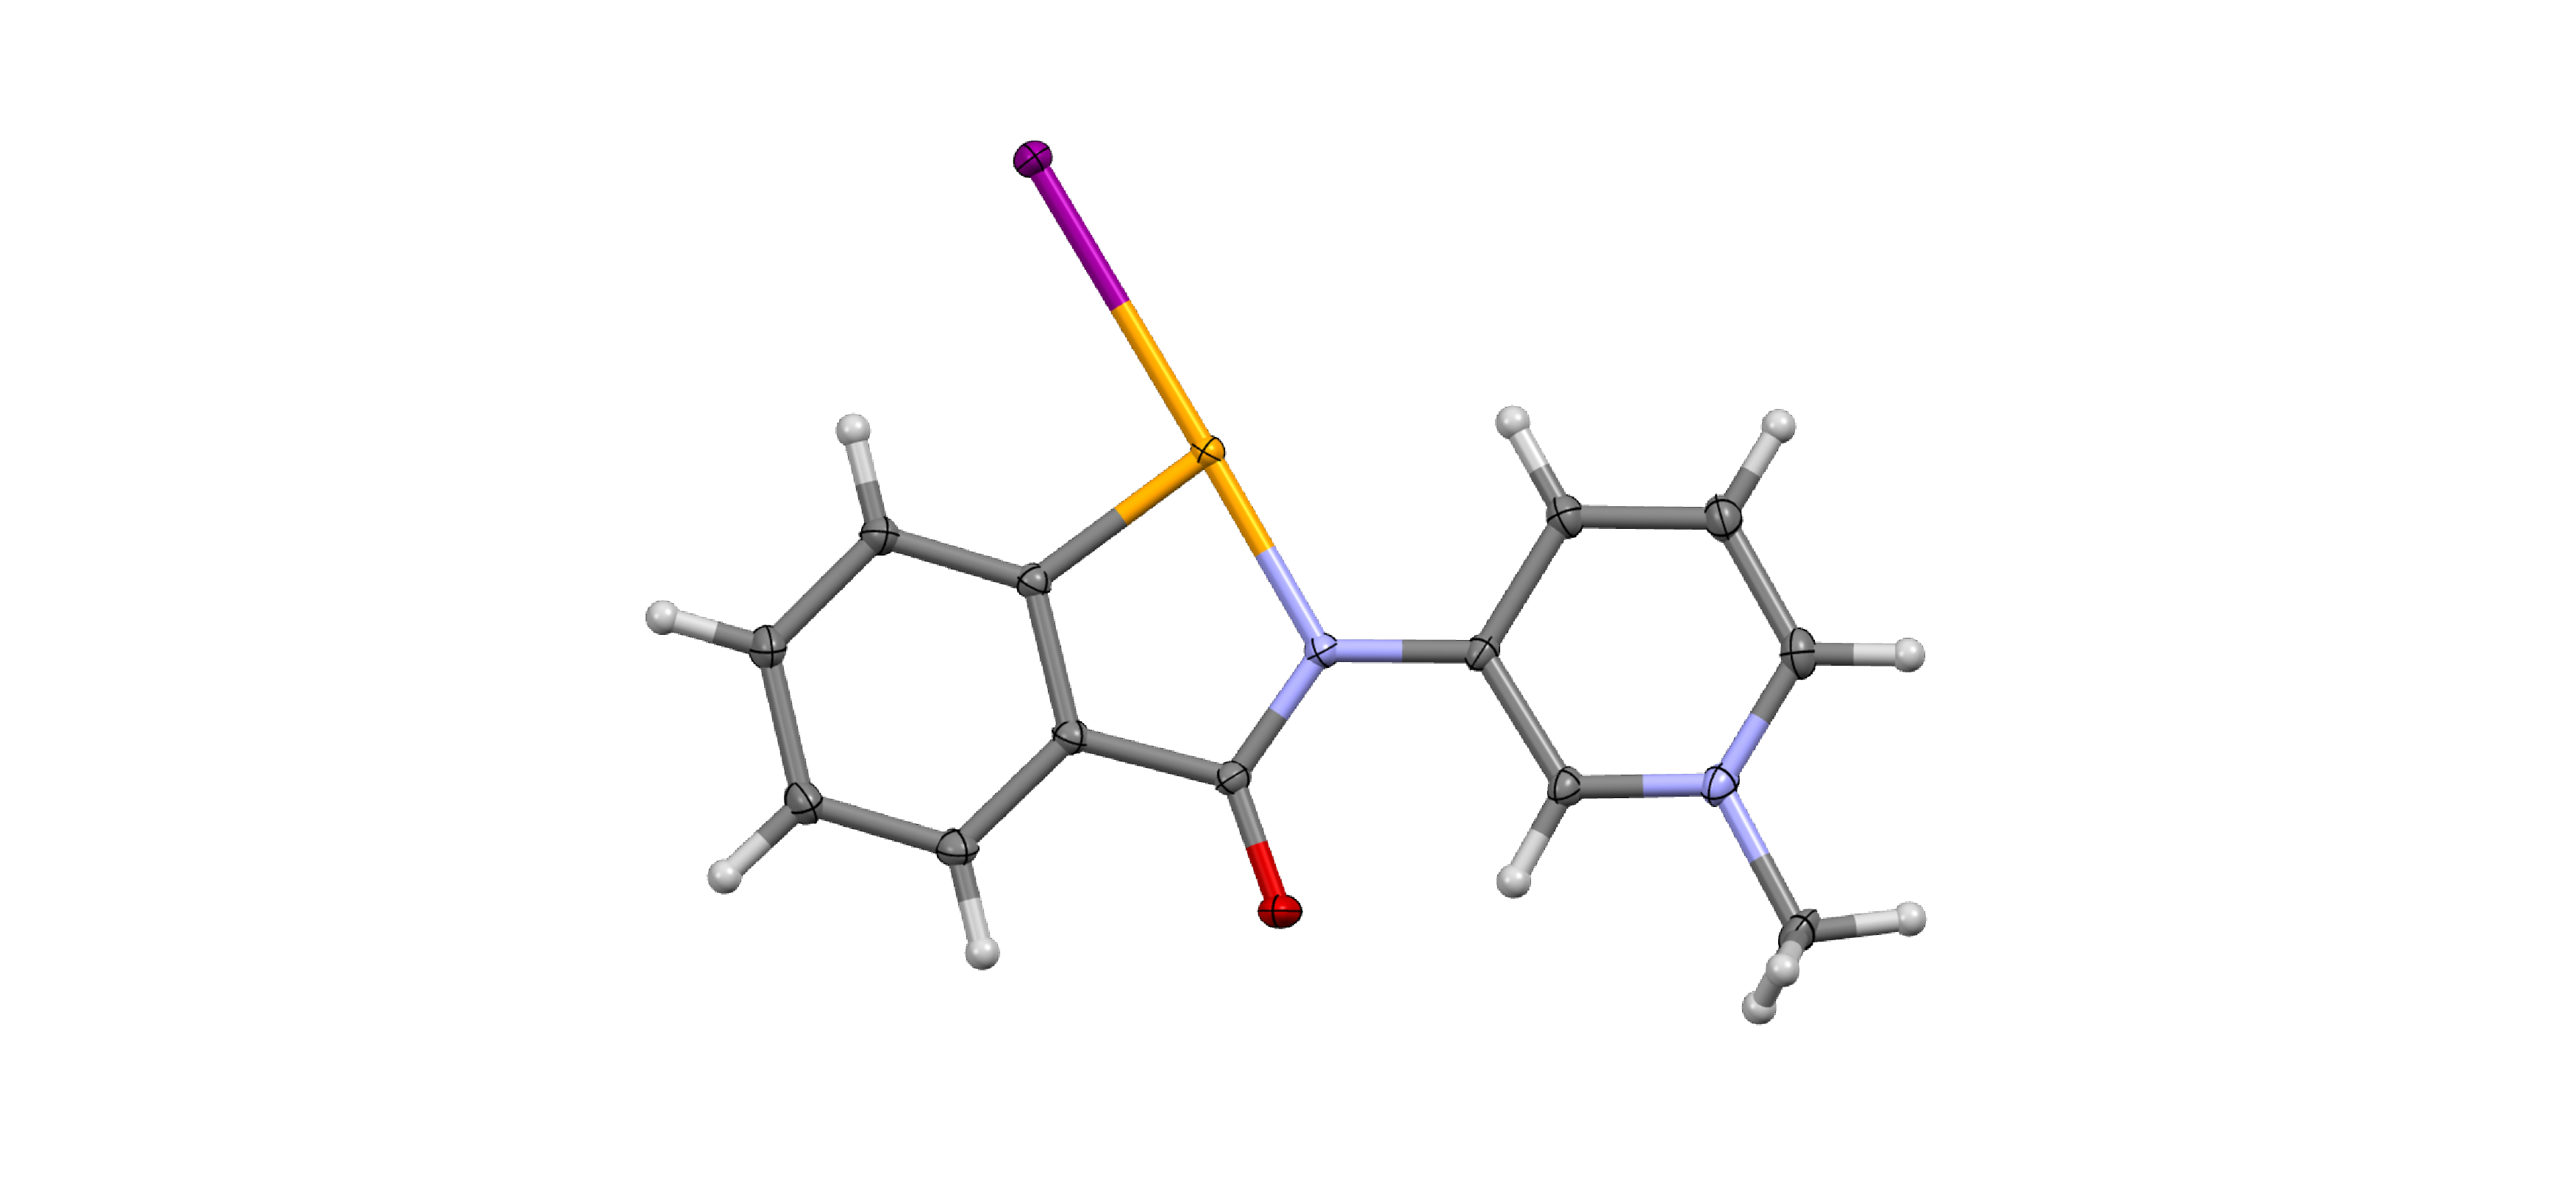
\includegraphics[width=\linewidth]{Figures/3py-ebs-mei.pdf}
        \caption{Structure of the methylated derivative \refcmpd{ebs.3pyme}.}
        \label{fig:3py-ebs-mei}
    \end{figure}
    
    In order to assess the effect of the positive charge on the Ch-bond, we required a system which lacked the charge on the ebselen molecule.
    We attempted to co-crystallise \cmpd{ebs.3py} with a variety of halide salts, but none gave the desired co-crystal.
    This is not entirely unsurprising, as most cations would not be easily incorporated in the lattice, disfavouring the formation of a co-crystal.
    However, when \cmpd{ebs.3py} was heated in aqueous \ce{HCl}, then slowly cooled, crystals of \cmpd{selenylchloride-3py} precipitated out of the solution (\cref{fig:3py-ebs-hcl}).
    The product \cmpd{selenylchloride-3py} corresponds to an extreme case of charge assisted Ch-bonding, where the endocyclic \ce{Se-N} bond is formally broken, and a new bond is established with the Ch-bond donor.
    We propose a mechanism for this transformation which involves protonation of the carbonyl oxygen by the strong acid, followed by nucleophilic attack by chloride at the selenium.
    The product then tautomerises to the more stable amide form, and an intramolecular Ch-bond is re-established, thus stabilising the selenyl chloride (\cref{sch:selenylchloride-mechanism}).
    The stability of this selenyl chloride is remarkable, as it is resistant to hydrolysis and oxidation, and may be kept in air for several weeks.
    
    \begin{figure}
        \centering
        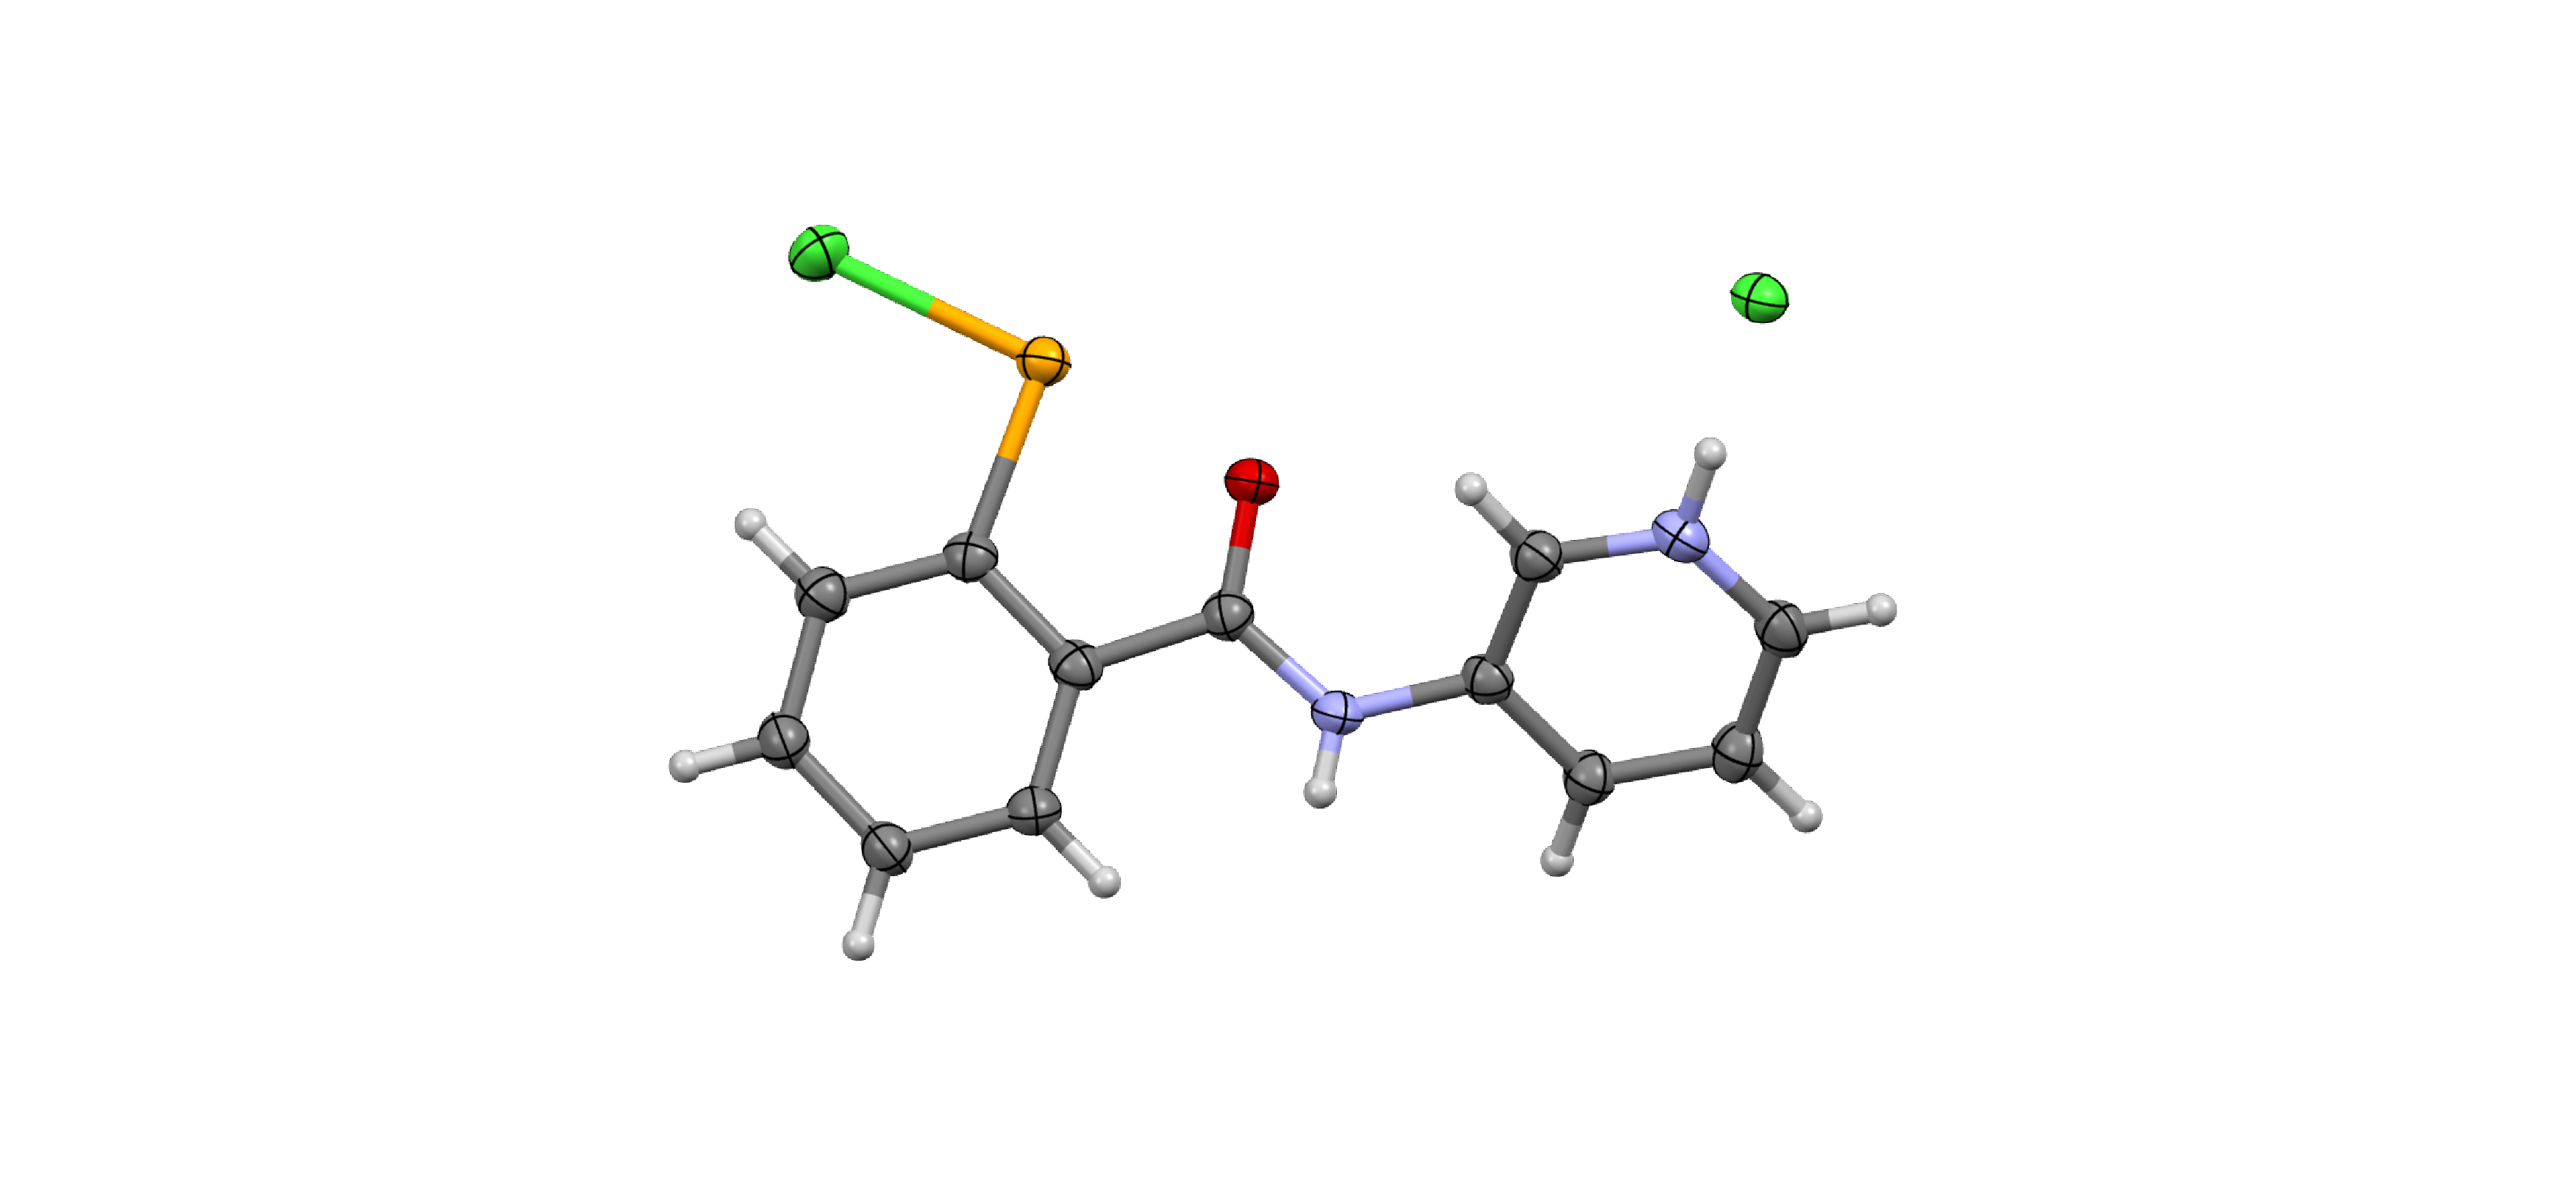
\includegraphics[width=\linewidth]{Figures/3py-ebs-hcl.pdf}
        \caption{Structure of the ring opened hydrochloride derivative \refcmpd{selenylchloride-3py}.}
        \label{fig:3py-ebs-hcl}
    \end{figure}
    
    \printbibliography[heading=subbibliography]
    
\end{refsection}
\end{comment}